\documentclass[border=4pt]{standalone}
\usepackage{fontspec}
\usepackage{amsmath}
\usepackage{unicode-math}
\setmainfont{Latin Modern Roman}
\setmathfont{Latin Modern Math}
\usepackage{pgfplots}
\usepackage{pgfplotstable}
\pgfplotsset{compat=1.18}
\usepackage{tkz-euclide}
\usetikzlibrary{arrows.meta,calc,angles,quotes,patterns,3d,backgrounds}
\definecolor{ink}{HTML}{123428}
\definecolor{asy}{HTML}{475569}
\definecolor{mint}{HTML}{86e0bd}
\tikzset{asym/.style={asy, line width=0.9pt, dash pattern=on 5pt off 3.5pt},
         guide/.style={gray!70, line width=0.6pt, densely dotted},
         dot/.style={circle, inner sep=0pt, minimum size=5pt, draw=white, line width=0.5pt},
         odot/.style={circle, inner sep=0pt, minimum size=5.5pt, fill=white, line width=1pt},
         lab/.style={font=\footnotesize, inner sep=1.5pt, text=ink}}
\begin{document}
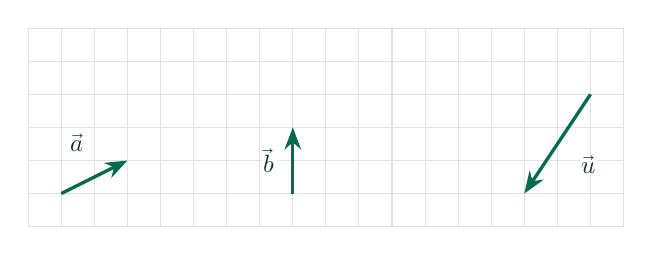
\begin{tikzpicture}
\draw[ink!14, line width=0.4pt] (0.000,0.000) -- (0.000,2.520);
\draw[ink!14, line width=0.4pt] (0.420,0.000) -- (0.420,2.520);
\draw[ink!14, line width=0.4pt] (0.840,0.000) -- (0.840,2.520);
\draw[ink!14, line width=0.4pt] (1.260,0.000) -- (1.260,2.520);
\draw[ink!14, line width=0.4pt] (1.680,0.000) -- (1.680,2.520);
\draw[ink!14, line width=0.4pt] (2.100,0.000) -- (2.100,2.520);
\draw[ink!14, line width=0.4pt] (2.520,0.000) -- (2.520,2.520);
\draw[ink!14, line width=0.4pt] (2.940,0.000) -- (2.940,2.520);
\draw[ink!14, line width=0.4pt] (3.360,0.000) -- (3.360,2.520);
\draw[ink!14, line width=0.4pt] (3.780,0.000) -- (3.780,2.520);
\draw[ink!14, line width=0.4pt] (4.200,0.000) -- (4.200,2.520);
\draw[ink!14, line width=0.4pt] (4.620,0.000) -- (4.620,2.520);
\draw[ink!14, line width=0.4pt] (5.040,0.000) -- (5.040,2.520);
\draw[ink!14, line width=0.4pt] (5.460,0.000) -- (5.460,2.520);
\draw[ink!14, line width=0.4pt] (5.880,0.000) -- (5.880,2.520);
\draw[ink!14, line width=0.4pt] (6.300,0.000) -- (6.300,2.520);
\draw[ink!14, line width=0.4pt] (6.720,0.000) -- (6.720,2.520);
\draw[ink!14, line width=0.4pt] (7.140,0.000) -- (7.140,2.520);
\draw[ink!14, line width=0.4pt] (7.560,0.000) -- (7.560,2.520);
\draw[ink!14, line width=0.4pt] (0.000,0.000) -- (7.560,0.000);
\draw[ink!14, line width=0.4pt] (0.000,0.420) -- (7.560,0.420);
\draw[ink!14, line width=0.4pt] (0.000,0.840) -- (7.560,0.840);
\draw[ink!14, line width=0.4pt] (0.000,1.260) -- (7.560,1.260);
\draw[ink!14, line width=0.4pt] (0.000,1.680) -- (7.560,1.680);
\draw[ink!14, line width=0.4pt] (0.000,2.100) -- (7.560,2.100);
\draw[ink!14, line width=0.4pt] (0.000,2.520) -- (7.560,2.520);
\draw[color={rgb,255:red,4;green,107;blue,77}, line width=1.2pt, -{Stealth[length=2.8mm]}] (0.420,0.420) -- (1.260,0.840);
\draw[color={rgb,255:red,4;green,107;blue,77}, line width=1.2pt, -{Stealth[length=2.8mm]}] (3.360,0.420) -- (3.360,1.260);
\draw[color={rgb,255:red,4;green,107;blue,77}, line width=1.2pt, -{Stealth[length=2.8mm]}] (7.140,1.680) -- (6.300,0.420);
\node[font=\small, text=ink, inner sep=0.5pt, fill=white] at (0.625,1.059) {$\vec a$};
\node[font=\small, text=ink, inner sep=0.5pt, fill=white] at (3.060,0.840) {$\vec b$};
\node[font=\small, text=ink, inner sep=0.5pt, fill=white] at (7.119,0.784) {$\vec u$};
\end{tikzpicture}
\end{document}
